\documentclass[1p]{elsarticle_modified}
%\bibliographystyle{elsarticle-num}

%\usepackage[colorlinks]{hyperref}
%\usepackage{abbrmath_seonhwa} %\Abb, \Ascr, \Acal ,\Abf, \Afrak
\usepackage{amsfonts}
\usepackage{amssymb}
\usepackage{amsmath}
\usepackage{amsthm}
\usepackage{scalefnt}
\usepackage{amsbsy}
\usepackage{kotex}
\usepackage{caption}
\usepackage{subfig}
\usepackage{color}
\usepackage{graphicx}
\usepackage{xcolor} %% white, black, red, green, blue, cyan, magenta, yellow
\usepackage{float}
\usepackage{setspace}
\usepackage{hyperref}

\usepackage{tikz}
\usetikzlibrary{arrows}

\usepackage{multirow}
\usepackage{array} % fixed length table
\usepackage{hhline}

%%%%%%%%%%%%%%%%%%%%%
\makeatletter
\renewcommand*\env@matrix[1][\arraystretch]{%
	\edef\arraystretch{#1}%
	\hskip -\arraycolsep
	\let\@ifnextchar\new@ifnextchar
	\array{*\c@MaxMatrixCols c}}
\makeatother %https://tex.stackexchange.com/questions/14071/how-can-i-increase-the-line-spacing-in-a-matrix
%%%%%%%%%%%%%%%

\usepackage[normalem]{ulem}

\newcommand{\msout}[1]{\ifmmode\text{\sout{\ensuremath{#1}}}\else\sout{#1}\fi}
%SOURCE: \msout is \stkout macro in https://tex.stackexchange.com/questions/20609/strikeout-in-math-mode

\newcommand{\cancel}[1]{
	\ifmmode
	{\color{red}\msout{#1}}
	\else
	{\color{red}\sout{#1}}
	\fi
}

\newcommand{\add}[1]{
	{\color{blue}\uwave{#1}}
}

\newcommand{\replace}[2]{
	\ifmmode
	{\color{red}\msout{#1}}{\color{blue}\uwave{#2}}
	\else
	{\color{red}\sout{#1}}{\color{blue}\uwave{#2}}
	\fi
}

\newcommand{\Sol}{\mathcal{S}} %segment
\newcommand{\D}{D} %diagram
\newcommand{\A}{\mathcal{A}} %arc


%%%%%%%%%%%%%%%%%%%%%%%%%%%%%5 test

\def\sl{\operatorname{\textup{SL}}(2,\Cbb)}
\def\psl{\operatorname{\textup{PSL}}(2,\Cbb)}
\def\quan{\mkern 1mu \triangleright \mkern 1mu}

\theoremstyle{definition}
\newtheorem{thm}{Theorem}[section]
\newtheorem{prop}[thm]{Proposition}
\newtheorem{lem}[thm]{Lemma}
\newtheorem{ques}[thm]{Question}
\newtheorem{cor}[thm]{Corollary}
\newtheorem{defn}[thm]{Definition}
\newtheorem{exam}[thm]{Example}
\newtheorem{rmk}[thm]{Remark}
\newtheorem{alg}[thm]{Algorithm}

\newcommand{\I}{\sqrt{-1}}
\begin{document}

%\begin{frontmatter}
%
%\title{Boundary parabolic representations of knots up to 8 crossings}
%
%%% Group authors per affiliation:
%\author{Yunhi Cho} 
%\address{Department of Mathematics, University of Seoul, Seoul, Korea}
%\ead{yhcho@uos.ac.kr}
%
%
%\author{Seonhwa Kim} %\fnref{s_kim}}
%\address{Center for Geometry and Physics, Institute for Basic Science, Pohang, 37673, Korea}
%\ead{ryeona17@ibs.re.kr}
%
%\author{Hyuk Kim}
%\address{Department of Mathematical Sciences, Seoul National University, Seoul 08826, Korea}
%\ead{hyukkim@snu.ac.kr}
%
%\author{Seokbeom Yoon}
%\address{Department of Mathematical Sciences, Seoul National University, Seoul, 08826,  Korea}
%\ead{sbyoon15@snu.ac.kr}
%
%\begin{abstract}
%We find all boundary parabolic representation of knots up to 8 crossings.
%
%\end{abstract}
%\begin{keyword}
%    \MSC[2010] 57M25 
%\end{keyword}
%
%\end{frontmatter}

%\linenumbers
%\tableofcontents
%
\newcommand\colored[1]{\textcolor{white}{\rule[-0.35ex]{0.8em}{1.4ex}}\kern-0.8em\color{red} #1}%
%\newcommand\colored[1]{\textcolor{white}{ #1}\kern-2.17ex	\textcolor{white}{ #1}\kern-1.81ex	\textcolor{white}{ #1}\kern-2.15ex\color{red}#1	}

{\Large $\underline{10_{101}~(K10a_{45})}$}

\setlength{\tabcolsep}{10pt}
\renewcommand{\arraystretch}{1.6}
\vspace{1cm}\begin{tabular}{m{100pt}>{\centering\arraybackslash}m{274pt}}
\multirow{5}{120pt}{
	\centering
	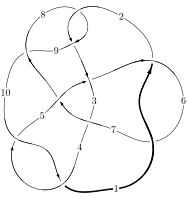
\includegraphics[width=112pt]{../../../GIT/diagram.site/Diagrams/png/185_10_101.png}\\
\ \ \ A knot diagram\footnotemark}&
\allowdisplaybreaks
\textbf{Linearized knot diagam} \\
\cline{2-2}
 &
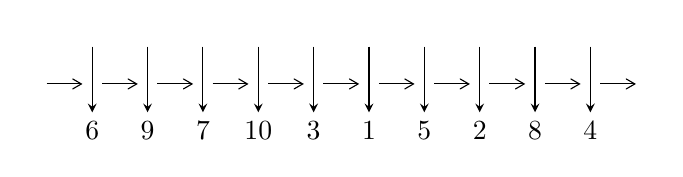
\begin{tikzpicture}[x=20pt, y=17pt]
	% nodes
	\node (C0) at (0, 0) {};
	\node (C1) at (1, 0) {};
	\node (C1U) at (1, +1) {};
	\node (C1D) at (1, -1) {6};

	\node (C2) at (2, 0) {};
	\node (C2U) at (2, +1) {};
	\node (C2D) at (2, -1) {9};

	\node (C3) at (3, 0) {};
	\node (C3U) at (3, +1) {};
	\node (C3D) at (3, -1) {7};

	\node (C4) at (4, 0) {};
	\node (C4U) at (4, +1) {};
	\node (C4D) at (4, -1) {10};

	\node (C5) at (5, 0) {};
	\node (C5U) at (5, +1) {};
	\node (C5D) at (5, -1) {3};

	\node (C6) at (6, 0) {};
	\node (C6U) at (6, +1) {};
	\node (C6D) at (6, -1) {1};

	\node (C7) at (7, 0) {};
	\node (C7U) at (7, +1) {};
	\node (C7D) at (7, -1) {5};

	\node (C8) at (8, 0) {};
	\node (C8U) at (8, +1) {};
	\node (C8D) at (8, -1) {2};

	\node (C9) at (9, 0) {};
	\node (C9U) at (9, +1) {};
	\node (C9D) at (9, -1) {8};

	\node (C10) at (10, 0) {};
	\node (C10U) at (10, +1) {};
	\node (C10D) at (10, -1) {4};
	\node (C11) at (11, 0) {};

	% arrows
	\draw[->,>={angle 60}]
	(C0) edge (C1) (C1) edge (C2) (C2) edge (C3) (C3) edge (C4) (C4) edge (C5) (C5) edge (C6) (C6) edge (C7) (C7) edge (C8) (C8) edge (C9) (C9) edge (C10) (C10) edge (C11) ;	\draw[->,>=stealth]
	(C1U) edge (C1D) (C2U) edge (C2D) (C3U) edge (C3D) (C4U) edge (C4D) (C5U) edge (C5D) (C6U) edge (C6D) (C7U) edge (C7D) (C8U) edge (C8D) (C9U) edge (C9D) (C10U) edge (C10D) ;
	\end{tikzpicture} \\
\hhline{~~} \\& 
\textbf{Solving Sequence} \\ \cline{2-2} 
 &
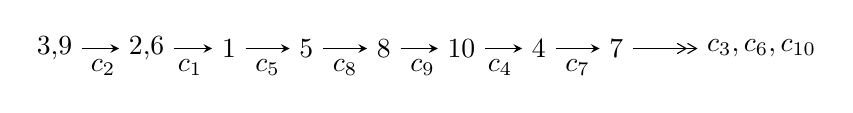
\begin{tikzpicture}[x=28pt, y=7pt]
	% node
	\node (A0) at (-1/8, 0) {3,9};
	\node (A1) at (17/16, 0) {2,6};
	\node (A2) at (17/8, 0) {1};
	\node (A3) at (25/8, 0) {5};
	\node (A4) at (33/8, 0) {8};
	\node (A5) at (41/8, 0) {10};
	\node (A6) at (49/8, 0) {4};
	\node (A7) at (57/8, 0) {7};
	\node (C1) at (1/2, -1) {$c_{2}$};
	\node (C2) at (13/8, -1) {$c_{1}$};
	\node (C3) at (21/8, -1) {$c_{5}$};
	\node (C4) at (29/8, -1) {$c_{8}$};
	\node (C5) at (37/8, -1) {$c_{9}$};
	\node (C6) at (45/8, -1) {$c_{4}$};
	\node (C7) at (53/8, -1) {$c_{7}$};
	\node (A8) at (9, 0) {$c_{3},c_{6},c_{10}$};

	% edge
	\draw[->,>=stealth]	
	(A0) edge (A1) (A1) edge (A2) (A2) edge (A3) (A3) edge (A4) (A4) edge (A5) (A5) edge (A6) (A6) edge (A7) ;
	\draw[->>,>={angle 60}]	
	(A7) edge (A8);
\end{tikzpicture} \\ 

\end{tabular} \\

\footnotetext{
The image of knot diagram is generated by the software ``\textbf{Draw programme}" developed by Andrew Bartholomew(\url{http://www.layer8.co.uk/maths/draw/index.htm\#Running-draw}), where we modified some parts for our purpose(\url{https://github.com/CATsTAILs/LinksPainter}).
}\phantom \\ \newline 
\centering \textbf{Ideals for irreducible components\footnotemark of $X_{\text{par}}$} 
 
\begin{align*}
I^u_{1}&=\langle 
7 u^{16}-32 u^{15}+\cdots+2 b+12,\;9 u^{16}-51 u^{15}+\cdots+2 a+43,\;u^{17}-6 u^{16}+\cdots+26 u-4\rangle \\
I^u_{2}&=\langle 
170 u^7 a^3-173 u^7 a^2+\cdots-479 a+513,\;2 u^7 a^3-11 u^7 a^2+\cdots-38 a+27,\\
\phantom{I^u_{2}}&\phantom{= \langle  }u^8+u^7- u^6-2 u^5+u^4+2 u^3-2 u-1\rangle \\
I^u_{3}&=\langle 
u^6-2 u^4+2 u^2+b+u-1,\;u^6- u^5- u^4+3 u^2+a-1,\;u^7- u^6- u^5+u^4+2 u^3- u^2- u+1\rangle \\
\\
\end{align*}
\raggedright * 3 irreducible components of $\dim_{\mathbb{C}}=0$, with total 56 representations.\\
\footnotetext{All coefficients of polynomials are rational numbers. But the coefficients are sometimes approximated in decimal forms when there is not enough margin.}
\newpage
\renewcommand{\arraystretch}{1}
\centering \section*{I. $I^u_{1}= \langle 7 u^{16}-32 u^{15}+\cdots+2 b+12,\;9 u^{16}-51 u^{15}+\cdots+2 a+43,\;u^{17}-6 u^{16}+\cdots+26 u-4 \rangle$}
\flushleft \textbf{(i) Arc colorings}\\
\begin{tabular}{m{7pt} m{180pt} m{7pt} m{180pt} }
\flushright $a_{3}=$&$\begin{pmatrix}1\\0\end{pmatrix}$ \\
\flushright $a_{9}=$&$\begin{pmatrix}0\\u\end{pmatrix}$ \\
\flushright $a_{2}=$&$\begin{pmatrix}1\\- u^2\end{pmatrix}$ \\
\flushright $a_{6}=$&$\begin{pmatrix}-\frac{9}{2} u^{16}+\frac{51}{2} u^{15}+\cdots+127 u-\frac{43}{2}\\-\frac{7}{2} u^{16}+16 u^{15}+\cdots+\frac{87}{2} u-6\end{pmatrix}$ \\
\flushright $a_{1}=$&$\begin{pmatrix}-\frac{9}{4} u^{16}+10 u^{15}+\cdots+\frac{95}{4} u-3\\\frac{3}{2} u^{16}-8 u^{15}+\cdots-\frac{79}{2} u+7\end{pmatrix}$ \\
\flushright $a_{5}=$&$\begin{pmatrix}-8 u^{16}+\frac{83}{2} u^{15}+\cdots+\frac{341}{2} u-\frac{55}{2}\\-\frac{7}{2} u^{16}+16 u^{15}+\cdots+\frac{87}{2} u-6\end{pmatrix}$ \\
\flushright $a_{8}=$&$\begin{pmatrix}u\\- u^3+u\end{pmatrix}$ \\
\flushright $a_{10}=$&$\begin{pmatrix}- u^3\\u^5- u^3+u\end{pmatrix}$ \\
\flushright $a_{4}=$&$\begin{pmatrix}- u^{16}+\frac{9}{2} u^{15}+\cdots+\frac{53}{2} u-\frac{7}{2}\\\frac{1}{2} u^{16}-2 u^{15}+\cdots+\frac{7}{2} u^2+\frac{1}{2} u\end{pmatrix}$ \\
\flushright $a_{7}=$&$\begin{pmatrix}-\frac{11}{4} u^{16}+15 u^{15}+\cdots+\frac{293}{4} u-12\\-\frac{3}{2} u^{16}+8 u^{15}+\cdots+\frac{65}{2} u-5\end{pmatrix}$\\&\end{tabular}
\flushleft \textbf{(ii) Obstruction class $= -1$}\\~\\
\flushleft \textbf{(iii) Cusp Shapes $= -15 u^{16}+81 u^{15}-169 u^{14}+62 u^{13}+429 u^{12}-933 u^{11}+562 u^{10}+878 u^9-2024 u^8+1325 u^7+679 u^6-1802 u^5+1076 u^4+221 u^3-663 u^2+360 u-78$}\\~\\
\newpage\renewcommand{\arraystretch}{1}
\flushleft \textbf{(iv) u-Polynomials at the component}\newline \\
\begin{tabular}{m{50pt}|m{274pt}}
Crossings & \hspace{64pt}u-Polynomials at each crossing \\
\hline $$\begin{aligned}c_{1},c_{4},c_{6}\\c_{10}\end{aligned}$$&$\begin{aligned}
&u^{17}+7 u^{15}+\cdots+u+1
\end{aligned}$\\
\hline $$\begin{aligned}c_{2},c_{8}\end{aligned}$$&$\begin{aligned}
&u^{17}+6 u^{16}+\cdots+26 u+4
\end{aligned}$\\
\hline $$\begin{aligned}c_{3}\end{aligned}$$&$\begin{aligned}
&u^{17}+18 u^{16}+\cdots+2816 u+256
\end{aligned}$\\
\hline $$\begin{aligned}c_{5},c_{7}\end{aligned}$$&$\begin{aligned}
&u^{17}+u^{16}+\cdots+6 u+1
\end{aligned}$\\
\hline $$\begin{aligned}c_{9}\end{aligned}$$&$\begin{aligned}
&u^{17}+6 u^{16}+\cdots+188 u+16
\end{aligned}$\\
\hline
\end{tabular}\\~\\
\newpage\renewcommand{\arraystretch}{1}
\flushleft \textbf{(v) Riley Polynomials at the component}\newline \\
\begin{tabular}{m{50pt}|m{274pt}}
Crossings & \hspace{64pt}Riley Polynomials at each crossing \\
\hline $$\begin{aligned}c_{1},c_{4},c_{6}\\c_{10}\end{aligned}$$&$\begin{aligned}
&y^{17}+14 y^{16}+\cdots+7 y-1
\end{aligned}$\\
\hline $$\begin{aligned}c_{2},c_{8}\end{aligned}$$&$\begin{aligned}
&y^{17}-6 y^{16}+\cdots+188 y-16
\end{aligned}$\\
\hline $$\begin{aligned}c_{3}\end{aligned}$$&$\begin{aligned}
&y^{17}+2 y^{16}+\cdots+524288 y-65536
\end{aligned}$\\
\hline $$\begin{aligned}c_{5},c_{7}\end{aligned}$$&$\begin{aligned}
&y^{17}+3 y^{16}+\cdots+6 y-1
\end{aligned}$\\
\hline $$\begin{aligned}c_{9}\end{aligned}$$&$\begin{aligned}
&y^{17}+10 y^{16}+\cdots+14704 y-256
\end{aligned}$\\
\hline
\end{tabular}\\~\\
\newpage\flushleft \textbf{(vi) Complex Volumes and Cusp Shapes}
$$\begin{array}{c|c|c}  
\text{Solutions to }I^u_{1}& \I (\text{vol} + \sqrt{-1}CS) & \text{Cusp shape}\\
 \hline 
\begin{aligned}
u &= -0.902416 + 0.208075 I \\
a &= -1.79366 - 0.59487 I \\
b &= \phantom{-}1.199630 + 0.242688 I\end{aligned}
 & -3.24705 + 0.67841 I & -12.7998 - 8.2767 I \\ \hline\begin{aligned}
u &= -0.902416 - 0.208075 I \\
a &= -1.79366 + 0.59487 I \\
b &= \phantom{-}1.199630 - 0.242688 I\end{aligned}
 & -3.24705 - 0.67841 I & -12.7998 + 8.2767 I \\ \hline\begin{aligned}
u &= \phantom{-}0.938877 + 0.582285 I \\
a &= -1.134880 + 0.826949 I \\
b &= \phantom{-}0.715526 + 0.898293 I\end{aligned}
 & -0.99442 - 4.22945 I & -12.33800 + 5.21456 I \\ \hline\begin{aligned}
u &= \phantom{-}0.938877 - 0.582285 I \\
a &= -1.134880 - 0.826949 I \\
b &= \phantom{-}0.715526 - 0.898293 I\end{aligned}
 & -0.99442 + 4.22945 I & -12.33800 - 5.21456 I \\ \hline\begin{aligned}
u &= \phantom{-}0.739806 + 0.493958 I \\
a &= \phantom{-}0.794662 - 0.257822 I \\
b &= \phantom{-}0.240261 - 0.634801 I\end{aligned}
 & -0.323057 - 0.236182 I & -11.08521 - 0.74956 I \\ \hline\begin{aligned}
u &= \phantom{-}0.739806 - 0.493958 I \\
a &= \phantom{-}0.794662 + 0.257822 I \\
b &= \phantom{-}0.240261 + 0.634801 I\end{aligned}
 & -0.323057 + 0.236182 I & -11.08521 + 0.74956 I \\ \hline\begin{aligned}
u &= \phantom{-}0.602874 + 0.959066 I \\
a &= -0.051648 - 0.335588 I \\
b &= -0.85046 + 1.32525 I\end{aligned}
 & \phantom{-}9.54876 + 8.47221 I & -3.97806 - 4.13044 I \\ \hline\begin{aligned}
u &= \phantom{-}0.602874 - 0.959066 I \\
a &= -0.051648 + 0.335588 I \\
b &= -0.85046 - 1.32525 I\end{aligned}
 & \phantom{-}9.54876 - 8.47221 I & -3.97806 + 4.13044 I \\ \hline\begin{aligned}
u &= \phantom{-}0.465319 + 1.172900 I \\
a &= -0.076760 + 0.308019 I \\
b &= \phantom{-}0.134443 - 0.808764 I\end{aligned}
 & \phantom{-}7.94985 - 2.22960 I & \phantom{-}2.70903 + 2.09494 I \\ \hline\begin{aligned}
u &= \phantom{-}0.465319 - 1.172900 I \\
a &= -0.076760 - 0.308019 I \\
b &= \phantom{-}0.134443 + 0.808764 I\end{aligned}
 & \phantom{-}7.94985 + 2.22960 I & \phantom{-}2.70903 - 2.09494 I\\
 \hline 
 \end{array}$$\newpage$$\begin{array}{c|c|c}  
\text{Solutions to }I^u_{1}& \I (\text{vol} + \sqrt{-1}CS) & \text{Cusp shape}\\
 \hline 
\begin{aligned}
u &= \phantom{-}1.101610 + 0.741547 I \\
a &= \phantom{-}1.82798 - 0.24157 I \\
b &= -1.09788 - 1.34726 I\end{aligned}
 & \phantom{-}7.9938 - 14.6875 I & -6.10908 + 8.19550 I \\ \hline\begin{aligned}
u &= \phantom{-}1.101610 - 0.741547 I \\
a &= \phantom{-}1.82798 + 0.24157 I \\
b &= -1.09788 + 1.34726 I\end{aligned}
 & \phantom{-}7.9938 + 14.6875 I & -6.10908 - 8.19550 I \\ \hline\begin{aligned}
u &= -1.311020 + 0.221936 I \\
a &= \phantom{-}0.907067 - 0.771746 I \\
b &= -0.650500 + 0.629679 I\end{aligned}
 & \phantom{-}1.56788 + 6.73537 I & -9.26043 - 8.18250 I \\ \hline\begin{aligned}
u &= -1.311020 - 0.221936 I \\
a &= \phantom{-}0.907067 + 0.771746 I \\
b &= -0.650500 - 0.629679 I\end{aligned}
 & \phantom{-}1.56788 - 6.73537 I & -9.26043 + 8.18250 I \\ \hline\begin{aligned}
u &= \phantom{-}1.18518 + 0.83889 I \\
a &= -0.962583 + 0.017371 I \\
b &= \phantom{-}0.662446 + 0.685312 I\end{aligned}
 & \phantom{-}5.79881 - 4.87487 I & -3.72990 + 6.85875 I \\ \hline\begin{aligned}
u &= \phantom{-}1.18518 - 0.83889 I \\
a &= -0.962583 - 0.017371 I \\
b &= \phantom{-}0.662446 - 0.685312 I\end{aligned}
 & \phantom{-}5.79881 + 4.87487 I & -3.72990 - 6.85875 I \\ \hline\begin{aligned}
u &= \phantom{-}0.359530\phantom{ +0.000000I} \\
a &= \phantom{-}0.979665\phantom{ +0.000000I} \\
b &= \phantom{-}0.293070\phantom{ +0.000000I}\end{aligned}
 & -0.661408\phantom{ +0.000000I} & -14.8170\phantom{ +0.000000I}\\
 \hline 
 \end{array}$$\newpage\newpage\renewcommand{\arraystretch}{1}
\centering \section*{II. $I^u_{2}= \langle 170 u^7 a^3-173 u^7 a^2+\cdots-479 a+513,\;2 u^7 a^3-11 u^7 a^2+\cdots-38 a+27,\;u^8+u^7- u^6-2 u^5+u^4+2 u^3-2 u-1 \rangle$}
\flushleft \textbf{(i) Arc colorings}\\
\begin{tabular}{m{7pt} m{180pt} m{7pt} m{180pt} }
\flushright $a_{3}=$&$\begin{pmatrix}1\\0\end{pmatrix}$ \\
\flushright $a_{9}=$&$\begin{pmatrix}0\\u\end{pmatrix}$ \\
\flushright $a_{2}=$&$\begin{pmatrix}1\\- u^2\end{pmatrix}$ \\
\flushright $a_{6}=$&$\begin{pmatrix}a\\-3.95349 a^{3} u^{7}+4.02326 a^{2} u^{7}+\cdots+11.1395 a-11.9302\end{pmatrix}$ \\
\flushright $a_{1}=$&$\begin{pmatrix}1.97674 a^{3} u^{7}-3.02326 a^{2} u^{7}+\cdots-13.0698 a+16.9302\\1.02326 a^{2} u^{7}-0.511628 u^{7}+\cdots-0.139535 a^{2}+1.06977\end{pmatrix}$ \\
\flushright $a_{5}=$&$\begin{pmatrix}-3.95349 a^{3} u^{7}+4.02326 a^{2} u^{7}+\cdots+12.1395 a-11.9302\\-3.95349 a^{3} u^{7}+4.02326 a^{2} u^{7}+\cdots+11.1395 a-11.9302\end{pmatrix}$ \\
\flushright $a_{8}=$&$\begin{pmatrix}u\\- u^3+u\end{pmatrix}$ \\
\flushright $a_{10}=$&$\begin{pmatrix}- u^3\\u^5- u^3+u\end{pmatrix}$ \\
\flushright $a_{4}=$&$\begin{pmatrix}-3 u^7 a^3+3 u^7 a^2+\cdots+12 a-13\\-2.04651 a^{3} u^{7}+1.97674 a^{2} u^{7}+\cdots+6.86047 a-8.06977\end{pmatrix}$ \\
\flushright $a_{7}=$&$\begin{pmatrix}3.06977 a^{3} u^{7}-2.95349 a^{2} u^{7}+\cdots-4.79070 a+4.13953\\2.04651 a^{3} u^{7}-1.97674 a^{2} u^{7}+\cdots-6.86047 a+7.06977\end{pmatrix}$\\&\end{tabular}
\flushleft \textbf{(ii) Obstruction class $= -1$}\\~\\
\flushleft \textbf{(iii) Cusp Shapes $= -\frac{352}{43} u^7 a^3+\frac{340}{43} u^7 a^2+\cdots+\frac{1180}{43} a-\frac{1818}{43}$}\\~\\
\newpage\renewcommand{\arraystretch}{1}
\flushleft \textbf{(iv) u-Polynomials at the component}\newline \\
\begin{tabular}{m{50pt}|m{274pt}}
Crossings & \hspace{64pt}u-Polynomials at each crossing \\
\hline $$\begin{aligned}c_{1},c_{4},c_{6}\\c_{10}\end{aligned}$$&$\begin{aligned}
&u^{32}+u^{31}+\cdots-10 u+1
\end{aligned}$\\
\hline $$\begin{aligned}c_{2},c_{8}\end{aligned}$$&$\begin{aligned}
&(u^8- u^7- u^6+2 u^5+u^4-2 u^3+2 u-1)^4
\end{aligned}$\\
\hline $$\begin{aligned}c_{3}\end{aligned}$$&$\begin{aligned}
&(u^2- u+1)^{16}
\end{aligned}$\\
\hline $$\begin{aligned}c_{5},c_{7}\end{aligned}$$&$\begin{aligned}
&u^{32}-9 u^{31}+\cdots-602 u+73
\end{aligned}$\\
\hline $$\begin{aligned}c_{9}\end{aligned}$$&$\begin{aligned}
&(u^8+3 u^7+7 u^6+10 u^5+11 u^4+10 u^3+6 u^2+4 u+1)^4
\end{aligned}$\\
\hline
\end{tabular}\\~\\
\newpage\renewcommand{\arraystretch}{1}
\flushleft \textbf{(v) Riley Polynomials at the component}\newline \\
\begin{tabular}{m{50pt}|m{274pt}}
Crossings & \hspace{64pt}Riley Polynomials at each crossing \\
\hline $$\begin{aligned}c_{1},c_{4},c_{6}\\c_{10}\end{aligned}$$&$\begin{aligned}
&y^{32}+27 y^{31}+\cdots+72 y+1
\end{aligned}$\\
\hline $$\begin{aligned}c_{2},c_{8}\end{aligned}$$&$\begin{aligned}
&(y^8-3 y^7+7 y^6-10 y^5+11 y^4-10 y^3+6 y^2-4 y+1)^4
\end{aligned}$\\
\hline $$\begin{aligned}c_{3}\end{aligned}$$&$\begin{aligned}
&(y^2+y+1)^{16}
\end{aligned}$\\
\hline $$\begin{aligned}c_{5},c_{7}\end{aligned}$$&$\begin{aligned}
&y^{32}+11 y^{31}+\cdots+23912 y+5329
\end{aligned}$\\
\hline $$\begin{aligned}c_{9}\end{aligned}$$&$\begin{aligned}
&(y^8+5 y^7+11 y^6+6 y^5-17 y^4-34 y^3-22 y^2-4 y+1)^4
\end{aligned}$\\
\hline
\end{tabular}\\~\\
\newpage\flushleft \textbf{(vi) Complex Volumes and Cusp Shapes}
$$\begin{array}{c|c|c}  
\text{Solutions to }I^u_{2}& \I (\text{vol} + \sqrt{-1}CS) & \text{Cusp shape}\\
 \hline 
\begin{aligned}
u &= -0.570868 + 0.730671 I \\
a &= \phantom{-}0.506748 + 0.672291 I \\
b &= -0.652472 + 0.678771 I\end{aligned}
 & \phantom{-}3.89415 + 0.89865 I & -5.41522 - 2.95331 I \\ \hline\begin{aligned}
u &= -0.570868 + 0.730671 I \\
a &= -0.193541 - 0.783831 I \\
b &= -0.485561 - 0.705520 I\end{aligned}
 & \phantom{-}3.89415 - 3.16112 I & -5.41522 + 3.97489 I \\ \hline\begin{aligned}
u &= -0.570868 + 0.730671 I \\
a &= \phantom{-}0.503876 - 0.375809 I \\
b &= \phantom{-}0.69485 + 1.61093 I\end{aligned}
 & \phantom{-}3.89415 - 3.16112 I & -5.41522 + 3.97489 I \\ \hline\begin{aligned}
u &= -0.570868 + 0.730671 I \\
a &= \phantom{-}0.342363 + 0.176286 I \\
b &= -0.236280 - 0.950229 I\end{aligned}
 & \phantom{-}3.89415 + 0.89865 I & -5.41522 - 2.95331 I \\ \hline\begin{aligned}
u &= -0.570868 - 0.730671 I \\
a &= \phantom{-}0.506748 - 0.672291 I \\
b &= -0.652472 - 0.678771 I\end{aligned}
 & \phantom{-}3.89415 - 0.89865 I & -5.41522 + 2.95331 I \\ \hline\begin{aligned}
u &= -0.570868 - 0.730671 I \\
a &= -0.193541 + 0.783831 I \\
b &= -0.485561 + 0.705520 I\end{aligned}
 & \phantom{-}3.89415 + 3.16112 I & -5.41522 - 3.97489 I \\ \hline\begin{aligned}
u &= -0.570868 - 0.730671 I \\
a &= \phantom{-}0.503876 + 0.375809 I \\
b &= \phantom{-}0.69485 - 1.61093 I\end{aligned}
 & \phantom{-}3.89415 + 3.16112 I & -5.41522 - 3.97489 I \\ \hline\begin{aligned}
u &= -0.570868 - 0.730671 I \\
a &= \phantom{-}0.342363 - 0.176286 I \\
b &= -0.236280 + 0.950229 I\end{aligned}
 & \phantom{-}3.89415 - 0.89865 I & -5.41522 + 2.95331 I \\ \hline\begin{aligned}
u &= \phantom{-}0.855237 + 0.665892 I \\
a &= -0.524115 - 0.290681 I \\
b &= \phantom{-}0.407531 - 1.001570 I\end{aligned}
 & \phantom{-}7.09422 - 0.54861 I & -2.27708 + 0.10386 I \\ \hline\begin{aligned}
u &= \phantom{-}0.855237 + 0.665892 I \\
a &= \phantom{-}0.10958 - 1.41649 I \\
b &= -1.60671 + 1.59050 I\end{aligned}
 & \phantom{-}7.09422 - 4.60838 I & -2.27708 + 7.03206 I\\
 \hline 
 \end{array}$$\newpage$$\begin{array}{c|c|c}  
\text{Solutions to }I^u_{2}& \I (\text{vol} + \sqrt{-1}CS) & \text{Cusp shape}\\
 \hline 
\begin{aligned}
u &= \phantom{-}0.855237 + 0.665892 I \\
a &= -2.13751 + 0.52423 I \\
b &= \phantom{-}0.473109 + 0.696143 I\end{aligned}
 & \phantom{-}7.09422 - 4.60838 I & -2.27708 + 7.03206 I \\ \hline\begin{aligned}
u &= \phantom{-}0.855237 + 0.665892 I \\
a &= \phantom{-}2.31080 - 1.01943 I \\
b &= -1.82102 - 1.12347 I\end{aligned}
 & \phantom{-}7.09422 - 0.54861 I & -2.27708 + 0.10386 I \\ \hline\begin{aligned}
u &= \phantom{-}0.855237 - 0.665892 I \\
a &= -0.524115 + 0.290681 I \\
b &= \phantom{-}0.407531 + 1.001570 I\end{aligned}
 & \phantom{-}7.09422 + 0.54861 I & -2.27708 - 0.10386 I \\ \hline\begin{aligned}
u &= \phantom{-}0.855237 - 0.665892 I \\
a &= \phantom{-}0.10958 + 1.41649 I \\
b &= -1.60671 - 1.59050 I\end{aligned}
 & \phantom{-}7.09422 + 4.60838 I & -2.27708 - 7.03206 I \\ \hline\begin{aligned}
u &= \phantom{-}0.855237 - 0.665892 I \\
a &= -2.13751 - 0.52423 I \\
b &= \phantom{-}0.473109 - 0.696143 I\end{aligned}
 & \phantom{-}7.09422 + 4.60838 I & -2.27708 - 7.03206 I \\ \hline\begin{aligned}
u &= \phantom{-}0.855237 - 0.665892 I \\
a &= \phantom{-}2.31080 + 1.01943 I \\
b &= -1.82102 + 1.12347 I\end{aligned}
 & \phantom{-}7.09422 + 0.54861 I & -2.27708 - 0.10386 I \\ \hline\begin{aligned}
u &= \phantom{-}1.09818\phantom{ +0.000000I} \\
a &= \phantom{-}1.40909 + 0.27112 I \\
b &= -0.797129 - 0.510365 I\end{aligned}
 & -1.56793 - 2.02988 I & -11.86404 + 3.46410 I \\ \hline\begin{aligned}
u &= \phantom{-}1.09818\phantom{ +0.000000I} \\
a &= \phantom{-}1.40909 - 0.27112 I \\
b &= -0.797129 + 0.510365 I\end{aligned}
 & -1.56793 + 2.02988 I & -11.86404 - 3.46410 I \\ \hline\begin{aligned}
u &= \phantom{-}1.09818\phantom{ +0.000000I} \\
a &= -0.79078 + 1.34206 I \\
b &= \phantom{-}0.736952 - 0.614594 I\end{aligned}
 & -1.56793 + 2.02988 I & -11.86404 - 3.46410 I \\ \hline\begin{aligned}
u &= \phantom{-}1.09818\phantom{ +0.000000I} \\
a &= -0.79078 - 1.34206 I \\
b &= \phantom{-}0.736952 + 0.614594 I\end{aligned}
 & -1.56793 - 2.02988 I & -11.86404 + 3.46410 I\\
 \hline 
 \end{array}$$\newpage$$\begin{array}{c|c|c}  
\text{Solutions to }I^u_{2}& \I (\text{vol} + \sqrt{-1}CS) & \text{Cusp shape}\\
 \hline 
\begin{aligned}
u &= -1.031810 + 0.655470 I \\
a &= \phantom{-}1.42398 + 0.08840 I \\
b &= -0.594791 + 0.693288 I\end{aligned}
 & \phantom{-}2.55512 + 4.41365 I & -7.42845 - 1.83007 I \\ \hline\begin{aligned}
u &= -1.031810 + 0.655470 I \\
a &= \phantom{-}1.24001 + 0.82764 I \\
b &= -0.595404 + 0.907218 I\end{aligned}
 & \phantom{-}2.55512 + 8.47342 I & -7.42845 - 8.75827 I \\ \hline\begin{aligned}
u &= -1.031810 + 0.655470 I \\
a &= -0.350327 + 0.360263 I \\
b &= -0.302783 - 0.841128 I\end{aligned}
 & \phantom{-}2.55512 + 4.41365 I & -7.42845 - 1.83007 I \\ \hline\begin{aligned}
u &= -1.031810 + 0.655470 I \\
a &= -2.16539 - 0.12217 I \\
b &= \phantom{-}1.17222 - 1.61062 I\end{aligned}
 & \phantom{-}2.55512 + 8.47342 I & -7.42845 - 8.75827 I \\ \hline\begin{aligned}
u &= -1.031810 - 0.655470 I \\
a &= \phantom{-}1.42398 - 0.08840 I \\
b &= -0.594791 - 0.693288 I\end{aligned}
 & \phantom{-}2.55512 - 4.41365 I & -7.42845 + 1.83007 I \\ \hline\begin{aligned}
u &= -1.031810 - 0.655470 I \\
a &= \phantom{-}1.24001 - 0.82764 I \\
b &= -0.595404 - 0.907218 I\end{aligned}
 & \phantom{-}2.55512 - 8.47342 I & -7.42845 + 8.75827 I \\ \hline\begin{aligned}
u &= -1.031810 - 0.655470 I \\
a &= -0.350327 - 0.360263 I \\
b &= -0.302783 + 0.841128 I\end{aligned}
 & \phantom{-}2.55512 - 4.41365 I & -7.42845 + 1.83007 I \\ \hline\begin{aligned}
u &= -1.031810 - 0.655470 I \\
a &= -2.16539 + 0.12217 I \\
b &= \phantom{-}1.17222 + 1.61062 I\end{aligned}
 & \phantom{-}2.55512 - 8.47342 I & -7.42845 + 8.75827 I \\ \hline\begin{aligned}
u &= -0.603304\phantom{ +0.000000I} \\
a &= \phantom{-}1.41265 + 0.18976 I \\
b &= -0.287361 + 1.327250 I\end{aligned}
 & \phantom{-}4.08977 - 2.02988 I & -9.89446 + 3.46410 I \\ \hline\begin{aligned}
u &= -0.603304\phantom{ +0.000000I} \\
a &= \phantom{-}1.41265 - 0.18976 I \\
b &= -0.287361 - 1.327250 I\end{aligned}
 & \phantom{-}4.08977 + 2.02988 I & -9.89446 - 3.46410 I\\
 \hline 
 \end{array}$$\newpage$$\begin{array}{c|c|c}  
\text{Solutions to }I^u_{2}& \I (\text{vol} + \sqrt{-1}CS) & \text{Cusp shape}\\
 \hline 
\begin{aligned}
u &= -0.603304\phantom{ +0.000000I} \\
a &= \phantom{-}0.40258 + 3.33383 I \\
b &= -0.605158 - 0.218634 I\end{aligned}
 & \phantom{-}4.08977 + 2.02988 I & -9.89446 - 3.46410 I \\ \hline\begin{aligned}
u &= -0.603304\phantom{ +0.000000I} \\
a &= \phantom{-}0.40258 - 3.33383 I \\
b &= -0.605158 + 0.218634 I\end{aligned}
 & \phantom{-}4.08977 - 2.02988 I & -9.89446 + 3.46410 I\\
 \hline 
 \end{array}$$\newpage\newpage\renewcommand{\arraystretch}{1}
\centering \section*{III. $I^u_{3}= \langle u^6-2 u^4+2 u^2+b+u-1,\;u^6- u^5- u^4+3 u^2+a-1,\;u^7- u^6- u^5+u^4+2 u^3- u^2- u+1 \rangle$}
\flushleft \textbf{(i) Arc colorings}\\
\begin{tabular}{m{7pt} m{180pt} m{7pt} m{180pt} }
\flushright $a_{3}=$&$\begin{pmatrix}1\\0\end{pmatrix}$ \\
\flushright $a_{9}=$&$\begin{pmatrix}0\\u\end{pmatrix}$ \\
\flushright $a_{2}=$&$\begin{pmatrix}1\\- u^2\end{pmatrix}$ \\
\flushright $a_{6}=$&$\begin{pmatrix}- u^6+u^5+u^4-3 u^2+1\\- u^6+2 u^4-2 u^2- u+1\end{pmatrix}$ \\
\flushright $a_{1}=$&$\begin{pmatrix}u^6- u^4- u^3+u^2+2 u+1\\u^5- u^3- u^2+u+1\end{pmatrix}$ \\
\flushright $a_{5}=$&$\begin{pmatrix}-2 u^6+u^5+3 u^4-5 u^2- u+2\\- u^6+2 u^4-2 u^2- u+1\end{pmatrix}$ \\
\flushright $a_{8}=$&$\begin{pmatrix}u\\- u^3+u\end{pmatrix}$ \\
\flushright $a_{10}=$&$\begin{pmatrix}- u^3\\u^5- u^3+u\end{pmatrix}$ \\
\flushright $a_{4}=$&$\begin{pmatrix}-2 u^6+u^5+2 u^4-4 u^2- u+2\\- u\end{pmatrix}$ \\
\flushright $a_{7}=$&$\begin{pmatrix}u^6- u^5-2 u^4+u^3+3 u^2-3\\u^6- u^5- u^4+2 u^2-1\end{pmatrix}$\\&\end{tabular}
\flushleft \textbf{(ii) Obstruction class $= 1$}\\~\\
\flushleft \textbf{(iii) Cusp Shapes $= -2 u^6+4 u^5+u^4- u^3-2 u^2+4 u-4$}\\~\\
\newpage\renewcommand{\arraystretch}{1}
\flushleft \textbf{(iv) u-Polynomials at the component}\newline \\
\begin{tabular}{m{50pt}|m{274pt}}
Crossings & \hspace{64pt}u-Polynomials at each crossing \\
\hline $$\begin{aligned}c_{1},c_{4}\end{aligned}$$&$\begin{aligned}
&u^7+4 u^5+u^4+6 u^3+2 u^2+4 u+1
\end{aligned}$\\
\hline $$\begin{aligned}c_{2}\end{aligned}$$&$\begin{aligned}
&u^7- u^6- u^5+u^4+2 u^3- u^2- u+1
\end{aligned}$\\
\hline $$\begin{aligned}c_{3}\end{aligned}$$&$\begin{aligned}
&u^7+u^6+u^5+u^4- u^2- u-1
\end{aligned}$\\
\hline $$\begin{aligned}c_{5},c_{7}\end{aligned}$$&$\begin{aligned}
&u^7- u^6+u^5- u^3+u^2- u+1
\end{aligned}$\\
\hline $$\begin{aligned}c_{6},c_{10}\end{aligned}$$&$\begin{aligned}
&u^7+4 u^5- u^4+6 u^3-2 u^2+4 u-1
\end{aligned}$\\
\hline $$\begin{aligned}c_{8}\end{aligned}$$&$\begin{aligned}
&u^7+u^6- u^5- u^4+2 u^3+u^2- u-1
\end{aligned}$\\
\hline $$\begin{aligned}c_{9}\end{aligned}$$&$\begin{aligned}
&u^7+3 u^6+7 u^5+9 u^4+10 u^3+7 u^2+3 u+1
\end{aligned}$\\
\hline
\end{tabular}\\~\\
\newpage\renewcommand{\arraystretch}{1}
\flushleft \textbf{(v) Riley Polynomials at the component}\newline \\
\begin{tabular}{m{50pt}|m{274pt}}
Crossings & \hspace{64pt}Riley Polynomials at each crossing \\
\hline $$\begin{aligned}c_{1},c_{4},c_{6}\\c_{10}\end{aligned}$$&$\begin{aligned}
&y^7+8 y^6+28 y^5+55 y^4+64 y^3+42 y^2+12 y-1
\end{aligned}$\\
\hline $$\begin{aligned}c_{2},c_{8}\end{aligned}$$&$\begin{aligned}
&y^7-3 y^6+7 y^5-9 y^4+10 y^3-7 y^2+3 y-1
\end{aligned}$\\
\hline $$\begin{aligned}c_{3}\end{aligned}$$&$\begin{aligned}
&y^7+y^6- y^5- y^4+2 y^3+y^2- y-1
\end{aligned}$\\
\hline $$\begin{aligned}c_{5},c_{7}\end{aligned}$$&$\begin{aligned}
&y^7+y^6- y^5-2 y^4+y^3+y^2- y-1
\end{aligned}$\\
\hline $$\begin{aligned}c_{9}\end{aligned}$$&$\begin{aligned}
&y^7+5 y^6+15 y^5+23 y^4+10 y^3-7 y^2-5 y-1
\end{aligned}$\\
\hline
\end{tabular}\\~\\
\newpage\flushleft \textbf{(vi) Complex Volumes and Cusp Shapes}
$$\begin{array}{c|c|c}  
\text{Solutions to }I^u_{3}& \I (\text{vol} + \sqrt{-1}CS) & \text{Cusp shape}\\
 \hline 
\begin{aligned}
u &= -0.793128 + 0.750889 I \\
a &= \phantom{-}0.905690 + 0.804408 I \\
b &= -0.888952 - 0.354053 I\end{aligned}
 & \phantom{-}6.43224 + 2.89342 I & -4.05142 - 2.86813 I \\ \hline\begin{aligned}
u &= -0.793128 - 0.750889 I \\
a &= \phantom{-}0.905690 - 0.804408 I \\
b &= -0.888952 + 0.354053 I\end{aligned}
 & \phantom{-}6.43224 - 2.89342 I & -4.05142 + 2.86813 I \\ \hline\begin{aligned}
u &= -0.879508\phantom{ +0.000000I} \\
a &= -1.71136\phantom{ +0.000000I} \\
b &= \phantom{-}1.06630\phantom{ +0.000000I}\end{aligned}
 & -3.03629\phantom{ +0.000000I} & -10.8170\phantom{ +0.000000I} \\ \hline\begin{aligned}
u &= \phantom{-}0.610619 + 0.459179 I \\
a &= \phantom{-}0.114923 - 1.389810 I \\
b &= -0.362477 - 1.085130 I\end{aligned}
 & \phantom{-}5.06800 + 1.30245 I & -2.75170 + 0.65887 I \\ \hline\begin{aligned}
u &= \phantom{-}0.610619 - 0.459179 I \\
a &= \phantom{-}0.114923 + 1.389810 I \\
b &= -0.362477 + 1.085130 I\end{aligned}
 & \phantom{-}5.06800 - 1.30245 I & -2.75170 - 0.65887 I \\ \hline\begin{aligned}
u &= \phantom{-}1.122260 + 0.611121 I \\
a &= -1.164940 - 0.276203 I \\
b &= \phantom{-}0.218278 + 0.857268 I\end{aligned}
 & \phantom{-}3.17738 - 5.75449 I & -4.78830 + 6.98275 I \\ \hline\begin{aligned}
u &= \phantom{-}1.122260 - 0.611121 I \\
a &= -1.164940 + 0.276203 I \\
b &= \phantom{-}0.218278 - 0.857268 I\end{aligned}
 & \phantom{-}3.17738 + 5.75449 I & -4.78830 - 6.98275 I\\
 \hline 
 \end{array}$$\newpage
\newpage\renewcommand{\arraystretch}{1}
\centering \section*{ IV. u-Polynomials}
\begin{tabular}{m{50pt}|m{274pt}}
Crossings & \hspace{64pt}u-Polynomials at each crossing \\
\hline $$\begin{aligned}c_{1},c_{4}\end{aligned}$$&$\begin{aligned}
&(u^7+4 u^5+u^4+6 u^3+2 u^2+4 u+1)(u^{17}+7 u^{15}+\cdots+u+1)\\
&\cdot(u^{32}+u^{31}+\cdots-10 u+1)
\end{aligned}$\\
\hline $$\begin{aligned}c_{2}\end{aligned}$$&$\begin{aligned}
&(u^7- u^6- u^5+u^4+2 u^3- u^2- u+1)\\
&\cdot((u^8- u^7+\cdots+2 u-1)^{4})(u^{17}+6 u^{16}+\cdots+26 u+4)
\end{aligned}$\\
\hline $$\begin{aligned}c_{3}\end{aligned}$$&$\begin{aligned}
&(u^2- u+1)^{16}(u^7+u^6+u^5+u^4- u^2- u-1)\\
&\cdot(u^{17}+18 u^{16}+\cdots+2816 u+256)
\end{aligned}$\\
\hline $$\begin{aligned}c_{5},c_{7}\end{aligned}$$&$\begin{aligned}
&(u^7- u^6+u^5- u^3+u^2- u+1)(u^{17}+u^{16}+\cdots+6 u+1)\\
&\cdot(u^{32}-9 u^{31}+\cdots-602 u+73)
\end{aligned}$\\
\hline $$\begin{aligned}c_{6},c_{10}\end{aligned}$$&$\begin{aligned}
&(u^7+4 u^5- u^4+6 u^3-2 u^2+4 u-1)(u^{17}+7 u^{15}+\cdots+u+1)\\
&\cdot(u^{32}+u^{31}+\cdots-10 u+1)
\end{aligned}$\\
\hline $$\begin{aligned}c_{8}\end{aligned}$$&$\begin{aligned}
&(u^7+u^6- u^5- u^4+2 u^3+u^2- u-1)\\
&\cdot((u^8- u^7+\cdots+2 u-1)^{4})(u^{17}+6 u^{16}+\cdots+26 u+4)
\end{aligned}$\\
\hline $$\begin{aligned}c_{9}\end{aligned}$$&$\begin{aligned}
&(u^7+3 u^6+7 u^5+9 u^4+10 u^3+7 u^2+3 u+1)\\
&\cdot(u^8+3 u^7+7 u^6+10 u^5+11 u^4+10 u^3+6 u^2+4 u+1)^4\\
&\cdot(u^{17}+6 u^{16}+\cdots+188 u+16)
\end{aligned}$\\
\hline
\end{tabular}\newpage\renewcommand{\arraystretch}{1}
\centering \section*{ V. Riley Polynomials}
\begin{tabular}{m{50pt}|m{274pt}}
Crossings & \hspace{64pt}Riley Polynomials at each crossing \\
\hline $$\begin{aligned}c_{1},c_{4},c_{6}\\c_{10}\end{aligned}$$&$\begin{aligned}
&(y^7+8 y^6+28 y^5+55 y^4+64 y^3+42 y^2+12 y-1)\\
&\cdot(y^{17}+14 y^{16}+\cdots+7 y-1)(y^{32}+27 y^{31}+\cdots+72 y+1)
\end{aligned}$\\
\hline $$\begin{aligned}c_{2},c_{8}\end{aligned}$$&$\begin{aligned}
&(y^7-3 y^6+7 y^5-9 y^4+10 y^3-7 y^2+3 y-1)\\
&\cdot(y^8-3 y^7+7 y^6-10 y^5+11 y^4-10 y^3+6 y^2-4 y+1)^4\\
&\cdot(y^{17}-6 y^{16}+\cdots+188 y-16)
\end{aligned}$\\
\hline $$\begin{aligned}c_{3}\end{aligned}$$&$\begin{aligned}
&(y^2+y+1)^{16}(y^7+y^6- y^5- y^4+2 y^3+y^2- y-1)\\
&\cdot(y^{17}+2 y^{16}+\cdots+524288 y-65536)
\end{aligned}$\\
\hline $$\begin{aligned}c_{5},c_{7}\end{aligned}$$&$\begin{aligned}
&(y^7+y^6+\cdots- y-1)(y^{17}+3 y^{16}+\cdots+6 y-1)\\
&\cdot(y^{32}+11 y^{31}+\cdots+23912 y+5329)
\end{aligned}$\\
\hline $$\begin{aligned}c_{9}\end{aligned}$$&$\begin{aligned}
&(y^7+5 y^6+15 y^5+23 y^4+10 y^3-7 y^2-5 y-1)\\
&\cdot(y^8+5 y^7+11 y^6+6 y^5-17 y^4-34 y^3-22 y^2-4 y+1)^4\\
&\cdot(y^{17}+10 y^{16}+\cdots+14704 y-256)
\end{aligned}$\\
\hline
\end{tabular}
\vskip 2pc
\end{document}